\documentclass{article}
\usepackage[utf8]{inputenc}
\usepackage{amsmath}
\usepackage{amsfonts}
\usepackage{mathrsfs}
\usepackage{graphicx}
\usepackage{subcaption}
\usepackage[top=20truemm,bottom=20truemm,left=20truemm,right=20truemm]{geometry}

\title{Chaotic Dynamics: Homework 8}
\author{Kansuke Ikehara (Kansuke.Ikehara@colorado.edu)}

\begin{document}
\maketitle

\subsection*{Problem 1}
Fig.\ref{q1a} shows a state-space trajectory of data1 constructed by divided difference.  In the process of reconstruction, data was \textit{undersampled} with the interval of 50 data points. If the interval was smaller, however, the reconstructed trajectory would look like having several lines horizontally.
\begin{figure}[h]
  \centering
  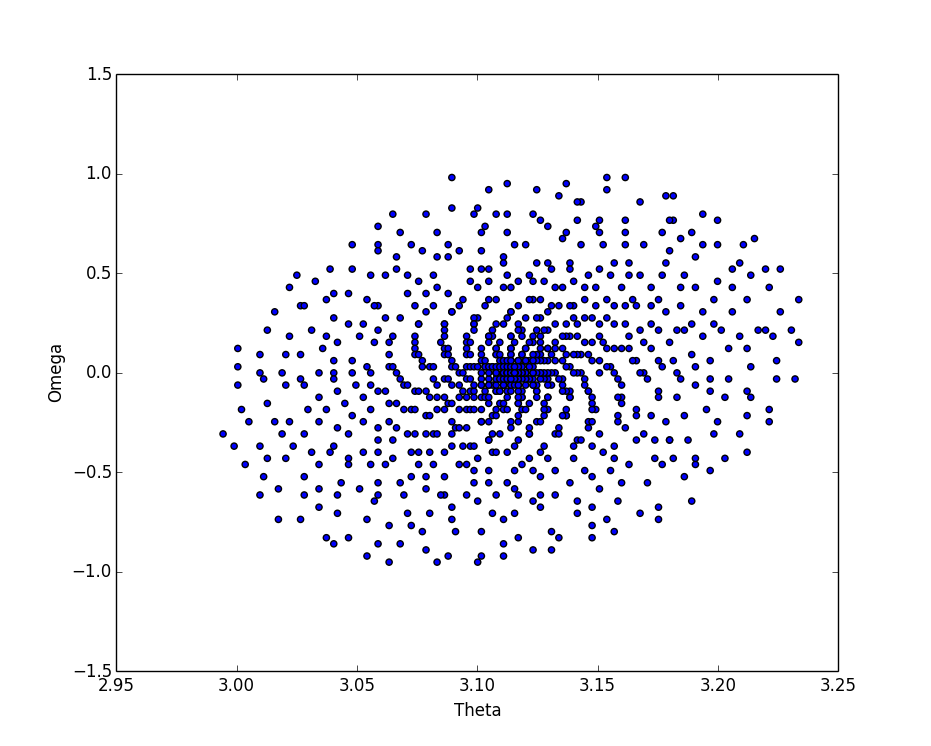
\includegraphics[height=2in]{figs/q1_interval_50.png}
  \caption{Constructed state-space trajectory by using divided difference.}
  \label{q1a}
\end{figure}

\subsection*{Problem 2}
\subsubsection*{(a)}
Fig.\ref{q2a} shows the constructed embedding of data2 with the conditions defined in (a). This embedding displays a chaotic attractor of a driven pendulum. 
\begin{figure}[h]
  \centering
  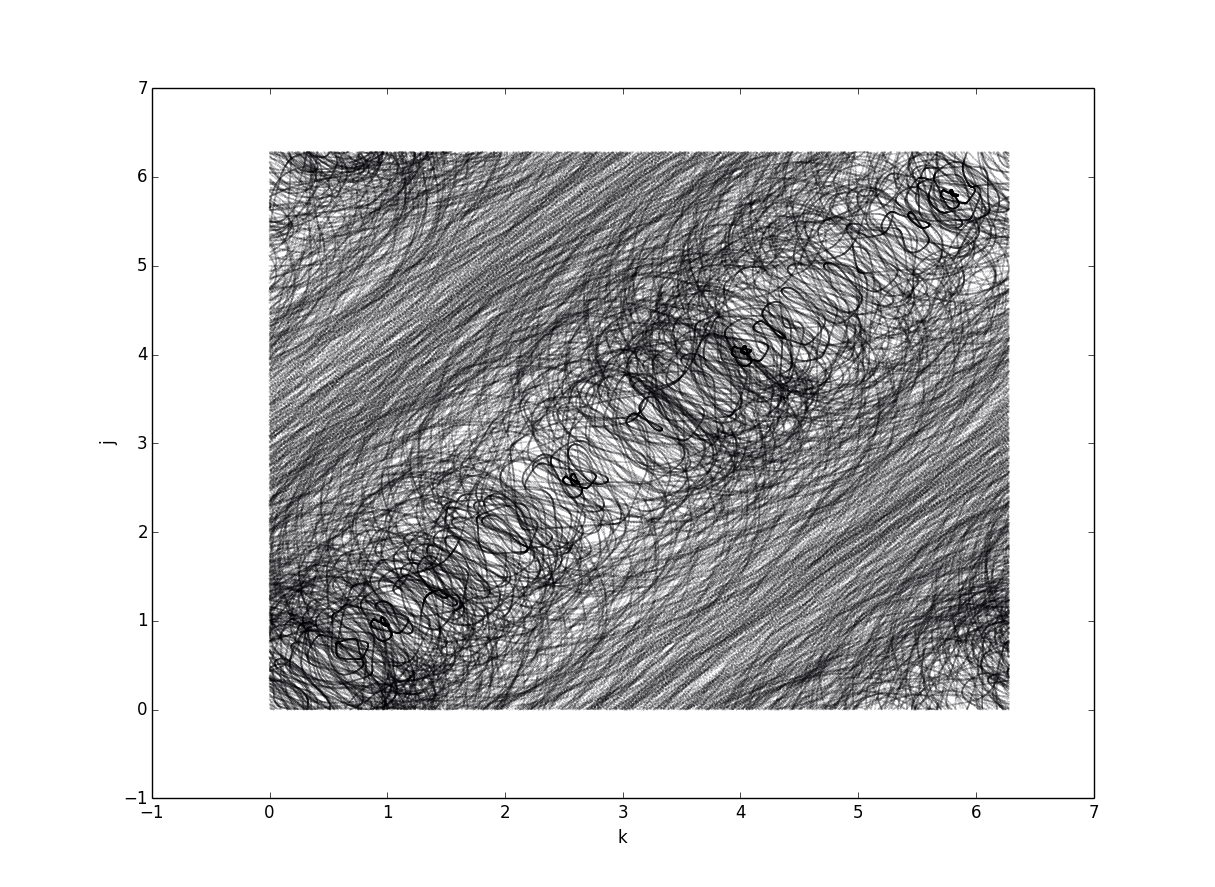
\includegraphics[height=2in]{figs/q2a.png}
  \caption{Reconstructed chaotic trajectory}
  \label{q2a}
\end{figure}

\subsubsection*{(b)}
Figs.\ref{q2b_1} and \ref{q2b_2} show the reconstructed state-space trajectories. As $\tau$ increases, the underlying dynamics gets unfolded as seen in fig.\ref{q2b_2}. The attractor is a periodic orbit.

\begin{figure}
\centering
\begin{subfigure}{.5\textwidth}
  \centering
  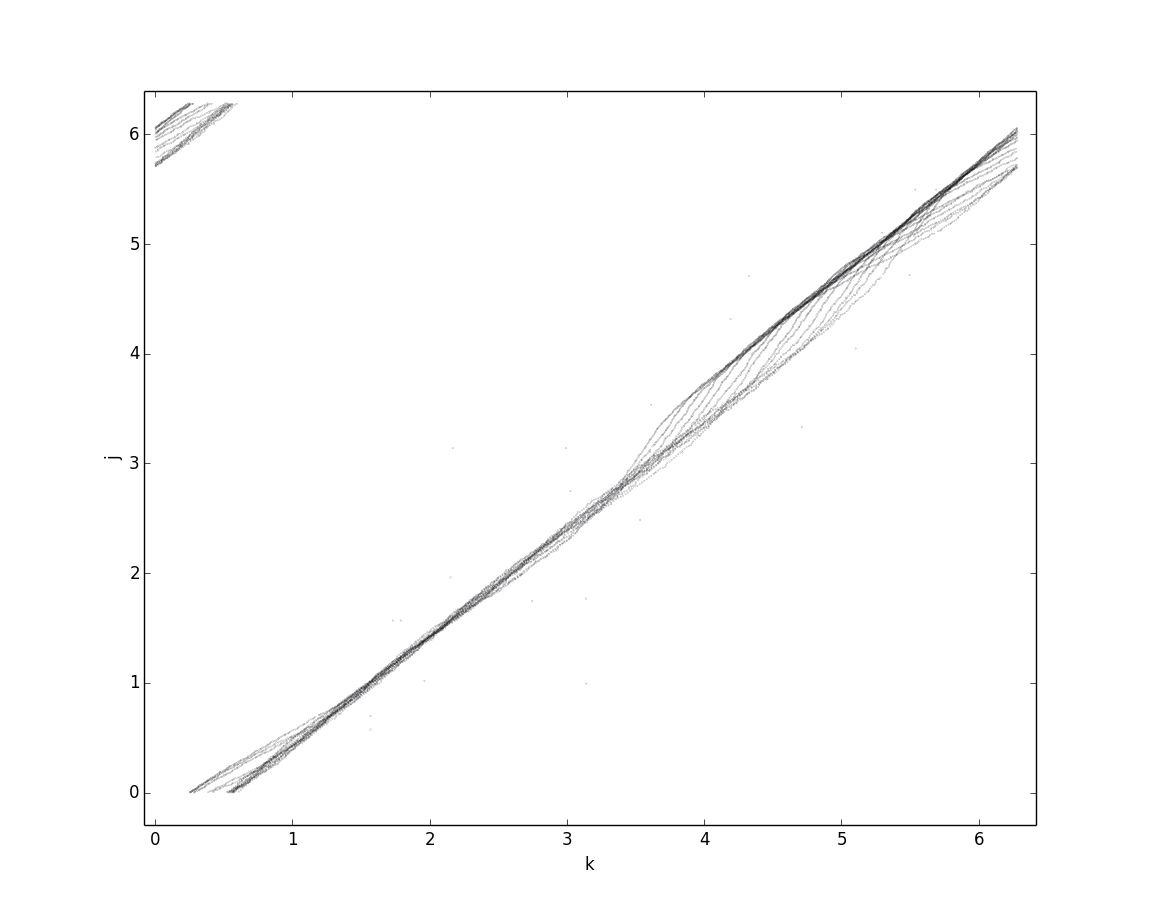
\includegraphics[height=2in]{figs/q2b_10.png}
  \caption{$\tau = 0.01$ sec}
  \label{q2b_1}
\end{subfigure}%
\begin{subfigure}{.5\textwidth}
  \centering
  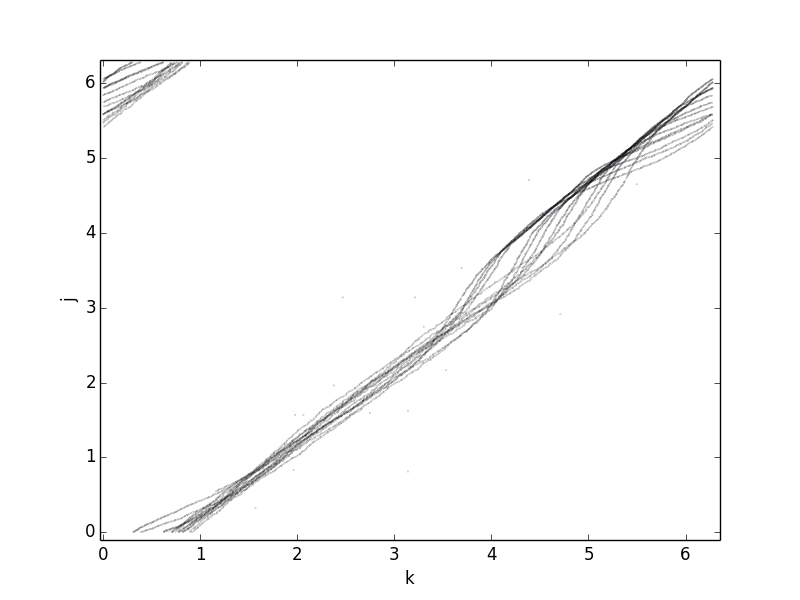
\includegraphics[height=2in]{figs/q2b_150.png}
  \caption{$\tau = 0.15$ sec}
  \label{q2b_2}
\end{subfigure}
\caption{Reconstructed state-space trajectory}
\label{q2b}
\end{figure}

\subsection*{Problem 3}
\subsubsection*{(a)}
Takens theorem states that in order to successfully reconstruct a topologically conjugate trajectory, one needs to satisfy the following:
\[
	m > 2d,
\]
where $m$ is the dimension of the reconstructed state-space and $d$ is the true dimension of the dynamics one is trying to reconstruct. Since driven pendulum has 3 dimensions in its dynamics: angle, angular velocity and angular velocity of driving force, we need $m = 7$ for successful embedding. For undriven pendulum, however, we only need $m = 5$ since its true dimension is 2: angle and angular velocity. 

\subsubsection*{(b)}
If $m = 2$, the resulting trajectory would look like a squashed form of the original trajectory since the dimension is too low and it has more points than one in a higher dimension. If $m = 25$, the trajectory would show its true form since we have a enough dimension to retain the original shape, but fewer points on the trajectory. 

\subsubsection*{(c)}
If $\tau$ was small, the reconstructed trajectory would basically be diagonal since sampled points are highly correlated. If $\tau$ was large, the trajectory would look like totally random, as sampled points are too far away from each other, resulting in no correlation.
\subsection*{Problem 4}
The first minimum of the curve of mutual information with respect to $\tau$ happens to be at the step $155$, which can be converted to $0.31$ second. The command line used to produce the output is as follows: \texttt{tisean-mutual ps8data/data2.first250sec -D 200 -o out.txt}

\begin{figure}[h]
  \centering
  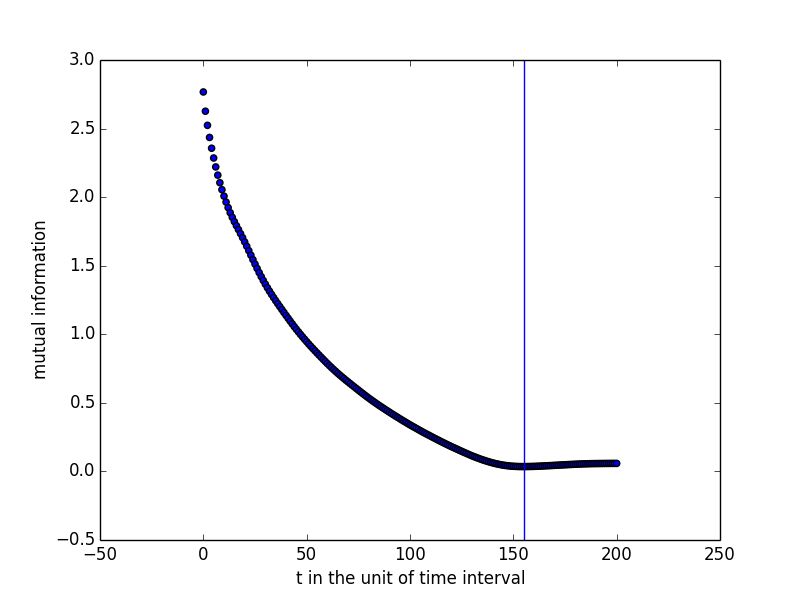
\includegraphics[height=2in]{figs/q4.png}
  \caption{Change of mutual information with respect to time delay}
  \label{q4}
  \end{figure}
  
\subsection*{Problem 5}
Fig.\ref{q5} shows the change of the ratio of false neighbors versus embedding dimension $m$. The first ratio which gets below 10\% (0.1) is at the dimension of $8$.  The command line used to produce the output is as follows: \texttt{tisean-false\_nearest ps8data/data2.first250sec -M 1,10 -d 155 -o false\_nearest.txt}


\begin{figure}[h]
  \centering
  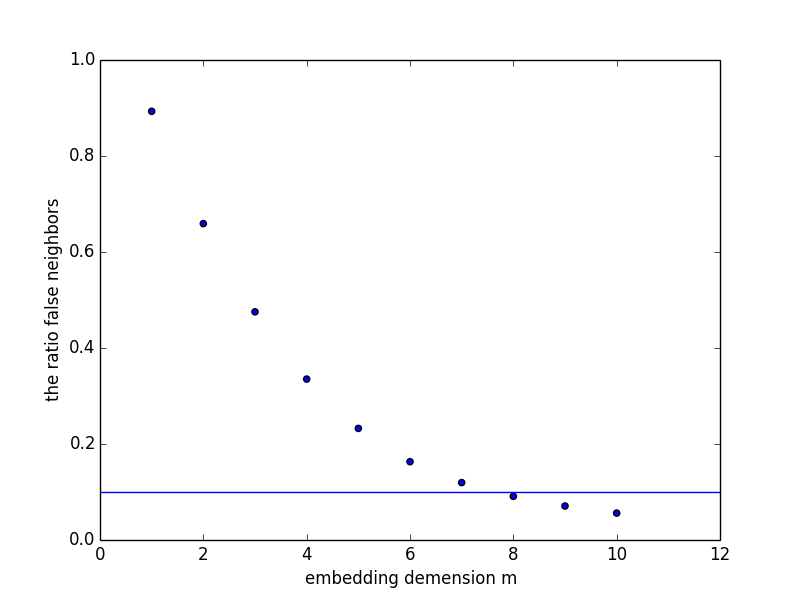
\includegraphics[height=2in]{figs/q5.png}
  \caption{The ratio of false neighbors versus embedding dimension $m$}
  \label{q5}
  \end{figure}
\end{document}












